\documentclass[14pt]{extarticle}
\usepackage{graphicx}
\usepackage{pslatex}
\usepackage[scaled]{helvet}

\usepackage{mathtools}

\usepackage{sfmath}  % Sans-serif math
\usepackage[a4paper, margin=0.8cm]{geometry}
\usepackage{amsmath}

\usepackage{sansmath}  % Use Helvetica for math symbols

\sansmath  % Activate sans-serif math font globally


\DeclareMathSizes{16}{14}{9}{7}

\renewcommand\familydefault{\sfdefault}

\renewcommand{\sfdefault}{phv}  % Use Helvetica for sans-serif
\everymath{\sf}  % Apply sans-serif font to all math expressions

\title{Triangle's Area}
\author{André Coelho}

\begin{document}
\maketitle





\begin{figure}[h]
\centering
  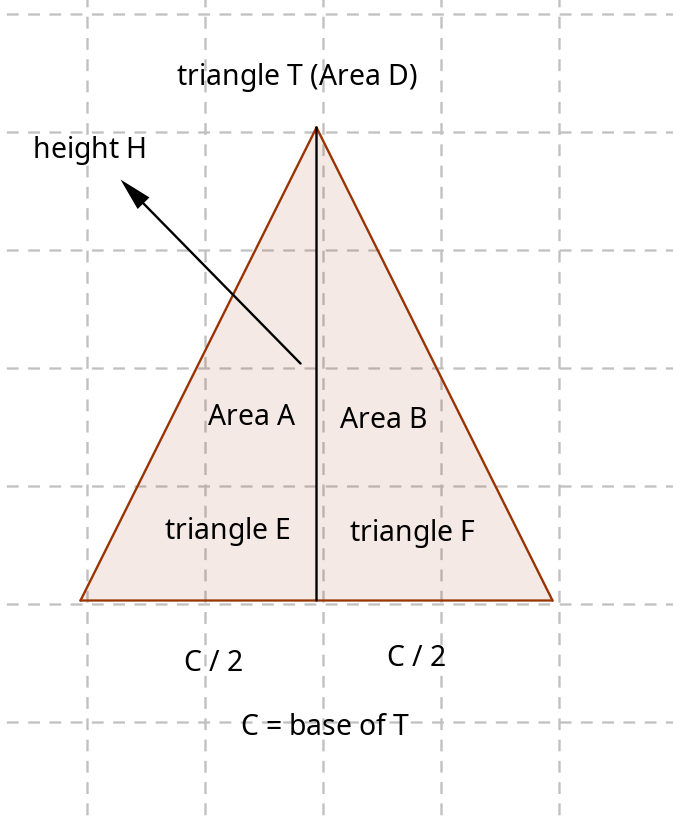
\includegraphics[width=0.5\textwidth]{triangle_area}
\end{figure}
 
 \begin{center}



Area Triangle = $ \dfrac{base}{2} * height $ \\[1cm]


2 * Area Triangle = $  base * height $ \\[1cm]
$Area\, D * 2 = base * height $ \\[1cm]
$base * height $ is the double of triangle's T area? \\[1cm]
Area A + Area B = Area D \\[1cm]
(Area A + Area B) * 2 = $ base * height $  \\[1cm]

Triangle T (with area D) has at least two triangles  \\[1cm]

Area A, has how many triangles?  \\[1cm]

Area A = $ \dfrac{C}{4} * height $  \\[1cm]

$ 2 * Area A = \dfrac{C}{2}  * height $  \\[1cm]

$ 4 * Area A = C * height $  \\[1cm]

C / 4 * height + C/ 4 * height = Area D  \\[1cm]

Area D = $ \dfrac{base * height}{2} = \dfrac{C}{4}  * height + \dfrac{C}{4} height $  \\[1cm]

H is the same for Area A and Area B, so Area D uses height,  but i have \( \dfrac{height}{2} \) , it will not be equal to Area of triangle T  \\[1cm]

\end{center}



\end{document}